% Condensed Part 3 (Adapting to Clinical Tasks). Two reused figures that both earn
% their place: the case-to-record schema (method, \input of the existing fragment)
% and the value-F1-vs-parameters plot (fig:p3-money, the result), copied verbatim
% from sources/part_3/chapter7. Prose is verbatim-cut from the abstract's Part-3
% paragraph and the capstone conclusion.

\noindent A clinical study keeps a structured form for each of its patients, the electronic
case report form, or eCRF. It holds one line per patient, with a fixed set of fields
such as the treatment given or the date it started, and it is filled from the
patient's own reports.

To turn these encoders into useful systems, we address the task that motivates this
thesis: extracting study-specific variables from clinical documents. Each project
asks for different fields, usually with little or no annotated data. No open
dataset pairs a French hospital record with a clinician-filled form, and the records
themselves cannot leave the hospital, so the supervision has to be built rather than
collected. We use large language models to annotate public text, to judge unseen
types when fixed references fall short, and to generate synthetic lymphoma dossiers
derived from clinical cases published in scientific articles. Both routes use
Qwen3-235B with constrained JSON output, and the resulting annotations are silver
rather than human labels.

\begin{center}
\begin{minipage}{\linewidth}
  \centering
  \resizebox{\textwidth}{!}{%
  \begin{tikzpicture}[
    font=\small, text=ThesisInk, >={Stealth[length=2mm]},
    box/.style={draw=ThesisNeutral, fill=ThesisPaper, rounded corners=3pt,
                text width=4.0cm, minimum height=3.3cm, inner sep=9pt, align=left},
    arr/.style={->, draw=ThesisNeutral, line width=0.7pt, shorten >=5pt, shorten <=5pt}]
    \node[box] (case) at (-5.0,0) {\textbf{Published case summary}\\[5pt]
      A patient was diagnosed with diffuse large B-cell lymphoma, received
      CHOEP-14, achieved remission, and relapsed fourteen years later.};
    \node[box] (timeline) at (0,0) {\textbf{Structured chronology}\\[6pt]
      \textcolor{ThesisPrimaryDark}{2018} · diagnosis\\
      \textcolor{ThesisPrimaryDark}{2018} · CHOEP-14\\
      \textcolor{ThesisPrimaryDark}{2019} · remission\\
      \textcolor{ThesisPrimaryDark}{2032} · relapse};
    \node[box] (reports) at (5.0,0) {\textbf{Generated French reports}\\[5pt]
      \textcolor{ThesisPrimaryDark}{18 May 2018} · pathology\\
      \textcolor{ThesisPrimaryDark}{22 May 2018} · tumour board\\
      \textcolor{ThesisPrimaryDark}{14 January 2019} · imaging\\
      \textcolor{ThesisPrimaryDark}{25 April 2032} · relapse visit};
    \draw[arr] (case) -- (timeline);
    \draw[arr] (timeline) -- (reports);
  \end{tikzpicture}}
  \captionof{figure}{Transformation of a fictional case summary into a dated longitudinal record.}
  \label{fig:p3-case-to-record}
\end{minipage}
\end{center}


\Cref{fig:p3-case-to-record} shows one such case and what we make of it: a published
case becomes a dated longitudinal record, a synthetic stand-in for the sequence of
reports a study form is filled from.

Generation follows the clinical chronology. We first convert the source case into a
structured French timeline, then generate the reports one at a time, extracting the
timeline again after each report as a consistency check, so that a report at a given
date receives only the events that have already occurred. The resulting corpus
contains 2,050 longitudinal records, each with a median of eight reports and 22,314
characters, and 31\% of them include a second treatment line. Turning these into an
extraction reference is a further step: each value must be linked to one of the 89
form fields and located in the complete record, and one language-model pass over
16,375 reports yields 237,194 span assignments across those fields. The reference is
silver, not human: the same model family generates the records and proposes their
labels, so it can reward the conventions of the generator rather than clinical
ground truth.

The generated supervision trains compact
open-vocabulary extractors whose target-field descriptions are supplied as text at
inference. On a synthetic eCRF benchmark, our smallest task-adapted model
outperforms extractive question answering and comes within 0.018 value-$F_1$ of the
strongest fine-tuned generator, a model twenty-seven times its size; a variant
adapted to the task closes the gap entirely, 0.657 against 0.658. Adaptation is also
data-efficient: value-$F_1$ rises from 0.182 with ten generated records to 0.485
with fifty and 0.659 with the full training set.

\begin{figure}[ht]
  \centering
  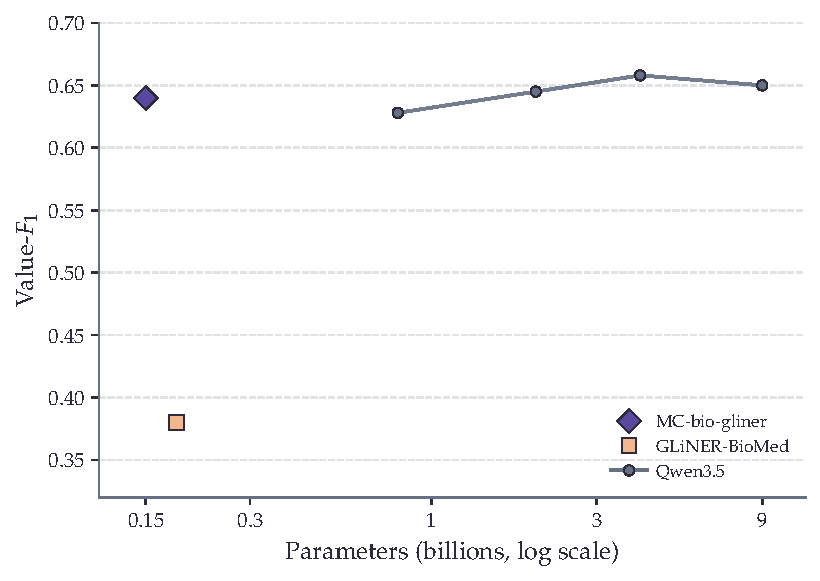
\includegraphics[width=0.82\textwidth]{plots/part_3/output/money_params_vs_f1.pdf}
  \caption{Value-$F_1$ on the lymphoma eCRF against parameter count, after field
  competition. The 150-million-parameter MC-bio-gliner comes within 0.018
  value-$F_1$ of the strongest generator Qwen3.5-4B at 27 times fewer parameters,
  while the size-matched GLiNER-BioMed baseline, fine-tuned on the same records,
  lags far behind.}
  \label{fig:p3-money}
\end{figure}

\Cref{fig:p3-money} places every system on the parameter axis. The task-adapted encoder
reaches the level of a four-billion-parameter generator, and scaling that generator
to nine billion does not help. The generators keep the advantage on span-$F_1$, up
to 0.567 against 0.503 for MC-bio-gliner, and among its errors the encoder assigns a
correct value to the wrong field 48.9\% of the time, against 38.8\% for the
strongest generator: more of its mistakes are role confusions, the right string
placed in the wrong slot.

The size gap is also a deployment gap. Confidentiality and the GDPR keep a
hospital's records off any external API, and the only on-site alternative, a
multi-billion-parameter generator, does not fit the modest hardware of a clinical
service. The encoder does: it runs where the data stays.

The synthetic eCRF measures the complete task but cannot establish transfer to
human-written text. On human NER sets (PARHAF, FRACCO), the advantage in fact narrows
to the longitudinal form-filling task the extractor was built for: on a dense, flat
NER task a size-matched baseline takes the lead again. Every part of this evidence is
synthetic or silver, with no real hospital record or human annotation in the task, so
whether the result carries to human-written records is the next thing to establish,
and the necessary step before any clinical use.
